%% Nepali multi-speaker TTS --- research paper
%% Compile: pdflatex paper.tex  (twice, for references). IEEEtran conference style.
%% Devanagari examples are romanized for portable typesetting (pdflatex-safe).
\documentclass[conference]{IEEEtran}
\IEEEoverridecommandlockouts
\usepackage[T1]{fontenc}
\usepackage{graphicx}
\usepackage{booktabs}
\usepackage{amsmath}
\usepackage{url}
\usepackage[hidelinks]{hyperref}

\begin{document}

\title{An Offline Multi-Speaker Nepali Text-to-Speech System on Consumer Hardware}

\author{\IEEEauthorblockN{Byapak Sigdel}
\IEEEauthorblockA{Independent Research \\
\texttt{github.com/ByapakSigdel/nepali-tts}}}

\maketitle

\begin{abstract}
We present a fully offline, multi-speaker Nepali (Devanagari) text-to-speech (TTS) system built entirely
from public data and trained on a single consumer 8\,GB laptop GPU. The system fine-tunes a VITS model
(via \emph{piper1-gpl}) from an English warm-start checkpoint, uses espeak-ng for Nepali
grapheme-to-phoneme (G2P) conversion, and exports to ONNX for dependency-light offline inference. Beyond the
model, we document a reproducible engineering recipe for training on a brand-new NVIDIA Blackwell
(\texttt{sm\_120}) laptop GPU under WSL2 with PyTorch~2.11 --- a configuration with several currently
undocumented failure modes. On approximately 3.8 hours of curated speech from 20 speakers, the generator loss
decreases monotonically (47 $\rightarrow$ 31) and the model produces increasingly intelligible Nepali across
multiple selectable voices. All code, configuration, and a clean-machine reproduction guide are released.
\end{abstract}

\begin{IEEEkeywords}
text-to-speech, Nepali, low-resource languages, VITS, multi-speaker, on-device inference, reproducibility
\end{IEEEkeywords}

\section{Introduction}
Nepali is a low-resource language for speech technology. High-quality TTS typically assumes (a) large clean
single-speaker corpora, (b) datacenter GPUs, and (c) online inference. We target the opposite regime:
\emph{public multi-speaker data, a single 8\,GB laptop GPU, and fully offline deployment}.

Our contributions are: (1) an end-to-end reproducible pipeline (data $\rightarrow$ preprocessing
$\rightarrow$ training $\rightarrow$ ONNX) for multi-speaker Nepali TTS; (2) a Nepali text frontend built on
espeak-ng with an empirical G2P accuracy analysis; (3) a documented engineering recipe for VITS training on
Blackwell\,+\,WSL2\,+\,PyTorch-2.11, which was the primary practical obstacle; and (4) full release of all
artifacts.

\section{Background and Components}
\textbf{VITS}~\cite{vits} is an end-to-end TTS model combining a conditional variational autoencoder,
normalizing flows, and adversarial training; it jointly learns acoustic representations and a HiFi-GAN-style
vocoder, supports multiple speakers via a learned speaker embedding, and reaches strong naturalness.
\textbf{Piper / piper1-gpl}~\cite{piper} is a lightweight VITS training and ONNX-inference toolkit aimed at
fast offline TTS; it provides espeak-ng phonemization and multi-speaker support.
\textbf{MMS-TTS}~\cite{mms} (\texttt{facebook/mms-tts-npl}) is a pretrained single-speaker Nepali VITS used
here as a baseline. \textbf{espeak-ng} is a rule-based multilingual phonemizer with a Nepali (\texttt{ne})
voice, used as our G2P frontend.

\section{Data}
We use public OpenSLR corpora (Table~\ref{tab:data}). The current \emph{Stage~A} corpus comprises 2{,}739
clips ($\sim$3.8 hours) from 20 speakers, resampled to 22.05\,kHz mono, peak-normalized, and silence-trimmed.
The corpus is heavily imbalanced (Fig.~\ref{fig:speakers}): the largest speaker contributes 566 clips, the
median about 60, and only one male speaker (109 clips) is present. Multi-speaker training shares phonetic
learning across all speakers, which mitigates but does not eliminate scarcity for data-poor voices.

\begin{table}[t]
\caption{Public OpenSLR corpora used.}
\label{tab:data}
\centering
\begin{tabular}{@{}llll@{}}
\toprule
ID & Content & License & Role \\
\midrule
SLR43  & Multi-speaker TTS (female) & CC BY-SA      & Stage A \\
SLR143 & TTS (male + female)        & CC BY-NC-SA   & Stage A \\
SLR54  & ASR, $\sim$157k utterances & CC BY-SA      & Stage B \\
\bottomrule
\end{tabular}
\end{table}

\begin{figure}[t]
\centering
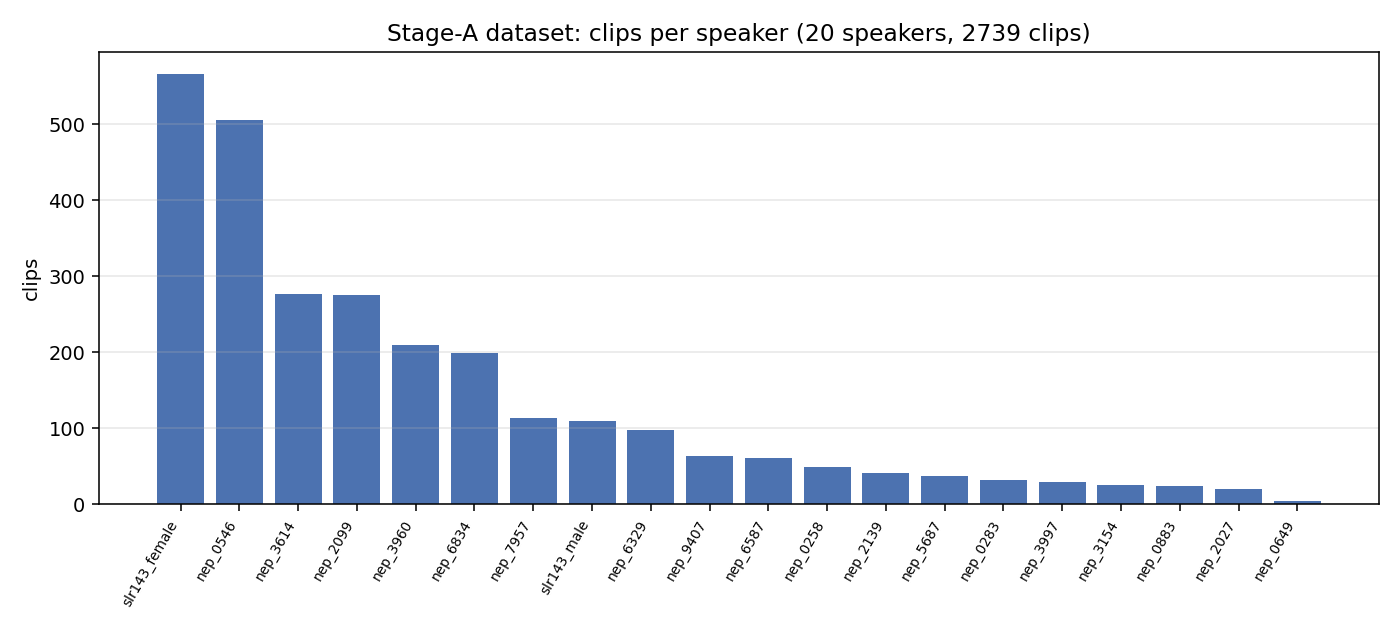
\includegraphics[width=\columnwidth]{dataset_speakers.png}
\caption{Clips per speaker in the Stage-A corpus (20 speakers, 2{,}739 clips).}
\label{fig:speakers}
\end{figure}

\begin{figure}[t]
\centering
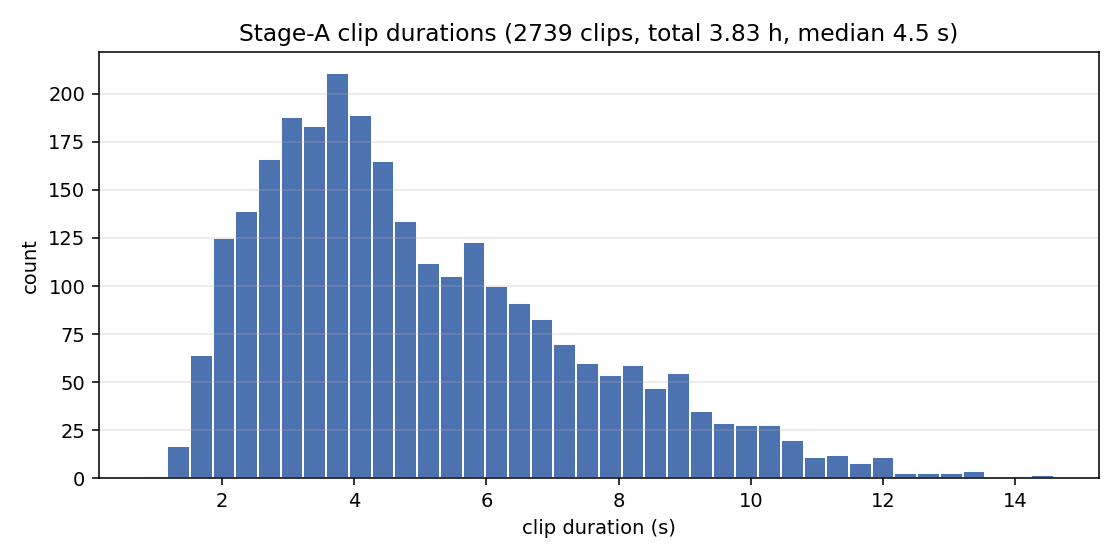
\includegraphics[width=\columnwidth]{duration_hist.png}
\caption{Clip-duration distribution of the Stage-A corpus; most clips fall in the 2--5\,s range.}
\label{fig:durations}
\end{figure}

\section{Method}
Figure~\ref{fig:pipeline} overviews the system: Nepali text is transliterated/phonemized in the frontend,
synthesized by a multi-speaker VITS model, exported to ONNX, and rendered to audio --- entirely offline.

\begin{figure*}[t]
\centering
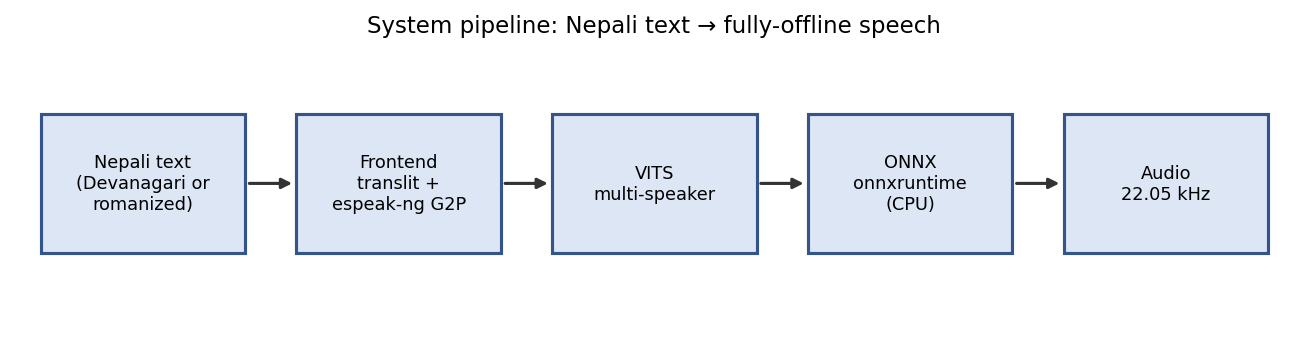
\includegraphics[width=\textwidth]{pipeline.png}
\caption{System pipeline: from Nepali text (Devanagari or romanized) to fully-offline speech.}
\label{fig:pipeline}
\end{figure*}

\subsection{Architecture}
We train a multi-speaker VITS model: the generator (SynthesizerTrn) has $\approx$30\,M parameters and the
multi-period discriminator $\approx$47\,M. A learned speaker embedding conditions the generator; voices are
selected at inference by integer speaker id.

\subsection{Nepali Text Frontend}
Devanagari text is converted to phonemes by espeak-ng (\texttt{ne}), a phoneme inventory of 256 symbols.
This handles consonant conjuncts, schwa, and numeral expansion natively (Section~\ref{sec:g2p}). Heavier
text normalization and a correction lexicon are left to future work.

\subsection{Warm-Start Transfer}
With only $\sim$3.8 hours of data, training from scratch is impractical on one GPU. We warm-start the vocoder
from the English \texttt{en\_US-lessac-medium} checkpoint: because VITS uses a shared IPA-based phoneme
inventory, the language-agnostic vocoder transfers while the model adapts to Nepali phonetics and speaker
identities. A full encoder/flow warm-start is blocked by the single$\rightarrow$multi-speaker architecture
mismatch and is future work.

\subsection{Offline Export}
Trained checkpoints are exported to ONNX (legacy exporter) and run via \texttt{onnxruntime} on CPU --- no GPU
or network required at inference. This is the deployable artifact.

\subsection{Deployment: Offline Web Frontend}
For interactive use we provide a Gradio web application (\texttt{frontend/app.py}). The user enters Nepali
text, selects one of the 20 speaker voices, optionally adjusts speed and variation, and receives audio. The
app loads the exported ONNX model, runs \texttt{onnxruntime} on CPU, and serves a browser UI on
\texttt{localhost} --- entirely offline; under WSL2 it is reachable from the Windows browser via
\texttt{localhost} forwarding. It re-exports the latest checkpoint on launch, so the served voice tracks
training progress. The app also accepts \emph{romanized} (Latin-script) Nepali and code-mixed English
(e.g.\ ``\textit{kasto cha tapaiko aaile}''): an offline rule transliterator
(\texttt{indic-transliteration}/OPTITRANS plus a curated Nepali word and phonetic-normalization map) converts
input to Devanagari, shown in an editable preview so the user can correct the residual errors of deterministic
transliteration before synthesis (Section~\ref{sec:future}).

\section{Experimental Setup}
Hardware and hyperparameters are summarized in Table~\ref{tab:setup}. Training runs unattended via an
auto-resume loop that checkpoints every 100 steps and restarts from the last checkpoint after any GPU fault.

\begin{table}[t]
\caption{Training configuration.}
\label{tab:setup}
\centering
\begin{tabular}{@{}ll@{}}
\toprule
Component & Value \\
\midrule
GPU & RTX 5050 Laptop, 8\,GB, Blackwell \texttt{sm\_120} \\
Stack & WSL2 Ubuntu-24.04, PyTorch 2.11+cu128, driver 610.47 \\
Precision & fp32 (\texttt{bf16}/\texttt{fp16} unusable; see App.~\ref{app:recipe}) \\
Batch size & 2, with 4 dataloader workers \\
Warm-start & \texttt{en\_US-lessac-medium} (vocoder) \\
Checkpointing & every 100 steps; fault-tolerant auto-resume \\
\bottomrule
\end{tabular}
\end{table}

\section{Results}
\subsection{Training Dynamics}
Figure~\ref{fig:losses} shows the generator (\texttt{loss\_g}) and discriminator (\texttt{loss\_d}) losses,
merged across all runs by training step. The generator loss falls sharply (47 $\rightarrow$ 37) within the
first few hundred steps as the warm-start adapts, then declines steadily to $\approx$31 by step 17.5k and
continues to trend downward. The discriminator loss remains balanced at $\approx$2.7 --- the expected stable
adversarial equilibrium, with no mode collapse or discriminator runaway.

\begin{figure}[t]
\centering
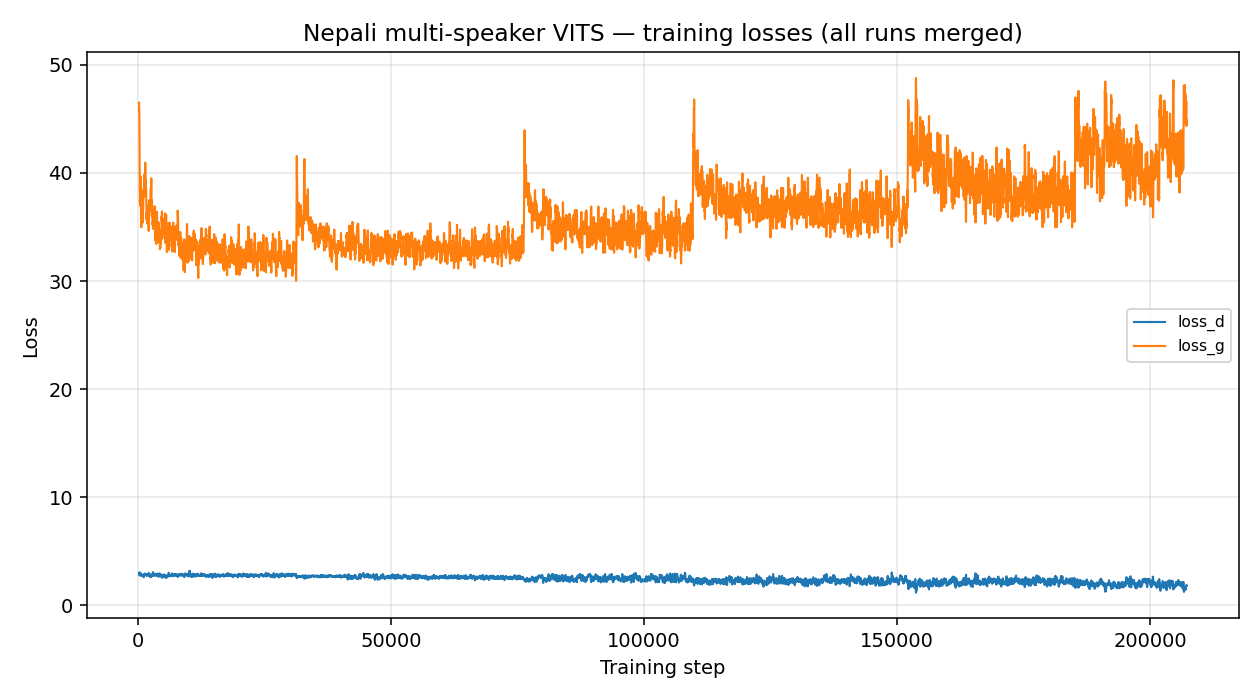
\includegraphics[width=\columnwidth]{training_losses.png}
\caption{Generator and discriminator losses (all runs merged by step).}
\label{fig:losses}
\end{figure}

\begin{figure}[t]
\centering
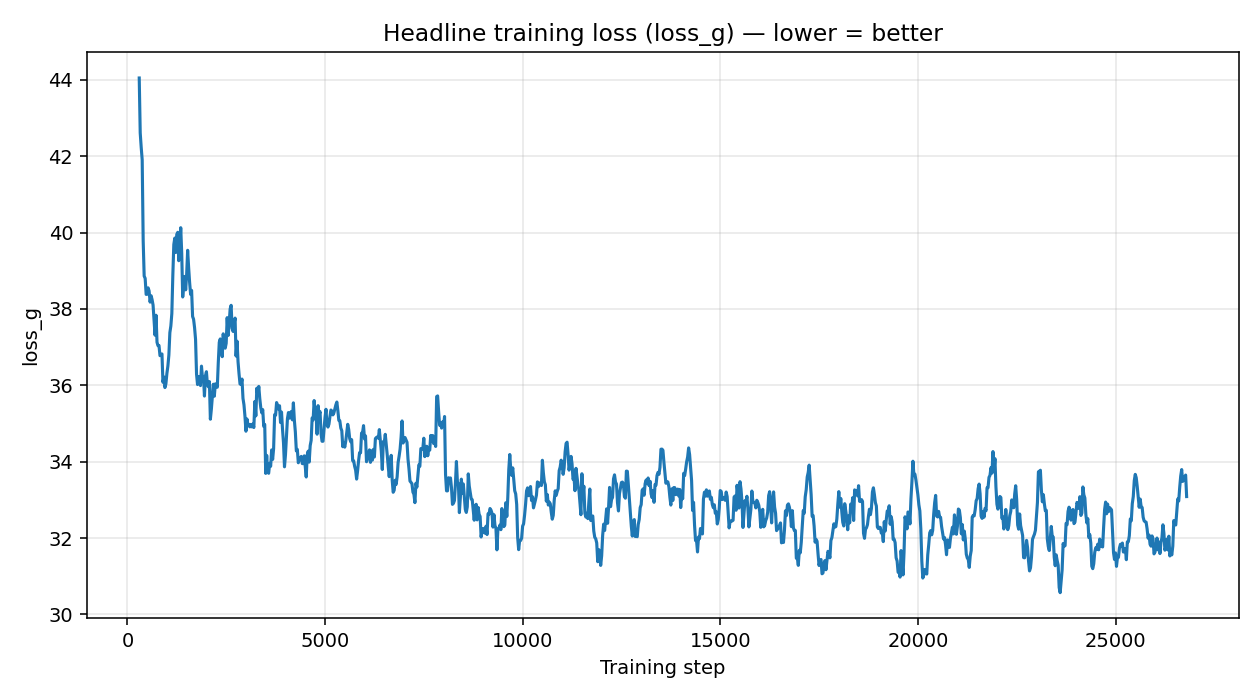
\includegraphics[width=\columnwidth]{headline_loss.png}
\caption{Generator loss alone: $47 \rightarrow 31$, still descending.}
\label{fig:headline}
\end{figure}

\subsection{Qualitative Output}
Figure~\ref{fig:mel} compares the mel-spectrogram of a ground-truth training clip against the model
synthesizing the \emph{same} utterance. The synthesized output reproduces the harmonic and formant structure
of natural speech --- evidence that the model has learned acoustic structure --- with the mildly smoothed
detail typical of mid-training.

\begin{figure*}[t]
\centering
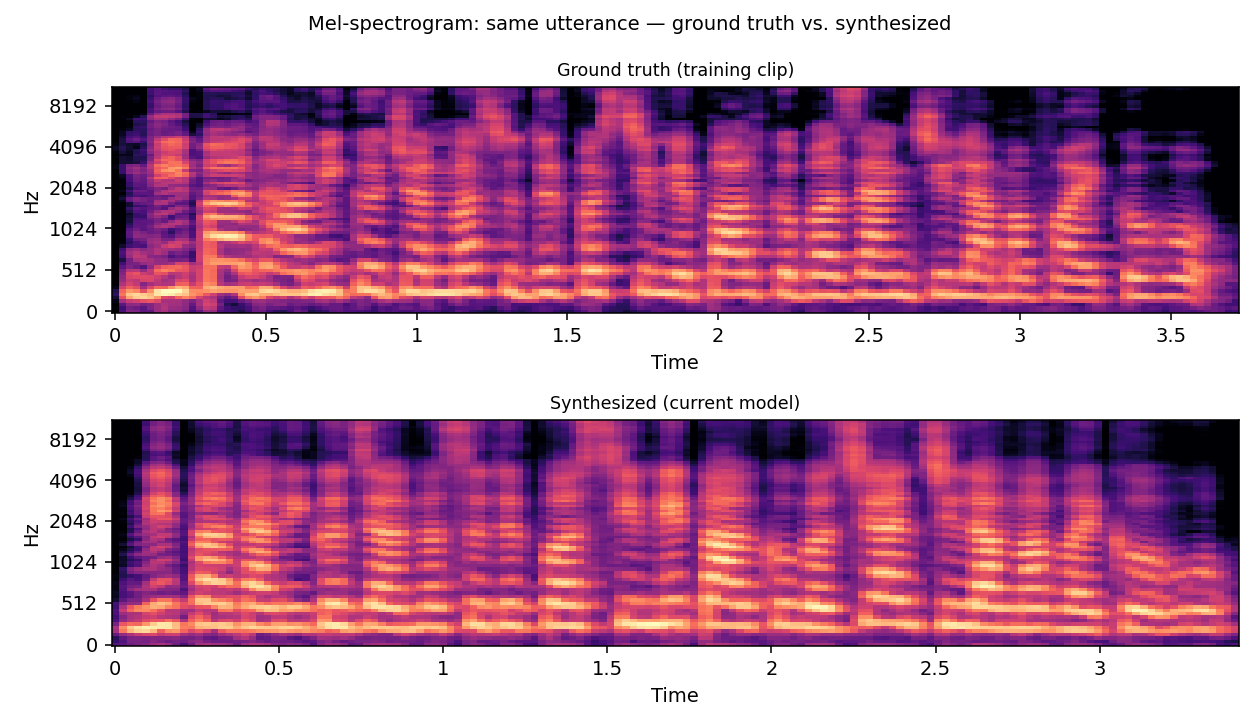
\includegraphics[width=0.92\textwidth]{mel_compare.png}
\caption{Mel-spectrograms of the same utterance: ground-truth training clip (top) vs.\ the current model
(bottom). The model recovers harmonics and formants; detail sharpens with further training.}
\label{fig:mel}
\end{figure*}

\subsection{G2P Frontend Accuracy}
\label{sec:g2p}
Table~\ref{tab:g2p} reports an empirical check of espeak-ng (\texttt{ne}) on representative inputs (romanized).
The frontend is largely correct; nasalization and a few phoneme nuances are the main targets for a future
correction lexicon.

\begin{table}[t]
\caption{espeak-ng (\texttt{ne}) G2P behavior on representative inputs.}
\label{tab:g2p}
\centering
\begin{tabular}{@{}lll@{}}
\toprule
Phenomenon & Example (romanized) & Verdict \\
\midrule
Consonant conjuncts & \emph{parikshan, vakya} & correct \\
Schwa deletion & \emph{namaste} & correct \\
Numeral expansion & 2026 $\rightarrow$ \emph{dui hajar chhabbis} & correct \\
Nasalization & \emph{tapaai, kathmandaum} & flattened \\
\bottomrule
\end{tabular}
\end{table}

\subsection{Objective Intelligibility (Methodology)}
Our planned objective metric is ASR round-trip Character Error Rate (CER): synthesize a held-out test set,
transcribe with a Nepali ASR (Whisper-large-v3 or MMS-ASR), and compute CER/WER against the input text.
Lower CER implies more intelligible output. The harness is implemented and released; because very early
checkpoints yield near-100\% CER, meaningful values are reported once the loss plateaus, against two
baselines: rule-based espeak-ng and neural MMS-tts-npl.

\section{Limitations and Future Work}
\label{sec:future}
The reported numbers are mid-training; quality and CER will improve. The corpus is small ($\sim$3.8\,h),
female-heavy, and has a single male voice; Stage~B (SLR54, $\sim$157k utterances) is expected to be the
largest quality lever. Planned work includes a Nepali normalization and correction lexicon (nasalization,
loanwords, dates, currency) and a deeper (encoder/flow) warm-start.

A second direction is \emph{input flexibility and code-switched naturalness}. Many Nepali speakers type in
Latin script (informal romanized Nepali) and freely mix English words, e.g.\ ``\textit{hello sanchai
hunuhuncha tapai}''. The frontend now transliterates informal romanized Nepali to Devanagari and handles
code-mixed Nepali-English tokens via a fully-offline rule transliterator, so users need not type Devanagari.
This is deliberately conservative: deterministic transliteration of orthography-free romanized Nepali tops out
near 80\% word accuracy (mitigated by the editable preview), and embedded English is rendered with a nativized
Nepali accent; replacing the rules with a small neural transliterator is a clean offline upgrade. Beyond
input, producing a genuinely natural, casually code-switched \emph{voice} (mirroring real Nepali-English
speech) is a modeling and data problem: it requires code-mixed training data and consistent phoneme handling
for embedded English words --- a longer-term research phase.

Finally, expressive/emotional TTS remains a separate phase, requiring emotion-labeled data that no public
Nepali corpus currently provides.

\section{Conclusion}
A reproducible, fully offline multi-speaker Nepali TTS system is achievable from public data on a single
8\,GB laptop GPU. The principal obstacle is not modeling but toolchain engineering on brand-new hardware,
which we document so others can reproduce it. Training is healthy and ongoing; the pipeline, data, and recipe
are released in full.

\appendices
\section{Reproducible Recipe: Blackwell (\texttt{sm\_120}) + WSL2 + PyTorch 2.11}
\label{app:recipe}
These failure modes are largely undocumented as of writing.
(1)~VITS's \texttt{@torch.jit.script} fused op crashes in the TorchScript interpreter on \texttt{sm\_120}
(mis-reported as a 20\,MiB OOM); set \texttt{PYTORCH\_JIT=0}.
(2)~\texttt{expandable\_segments:True} uses CUDA virtual-memory APIs unsupported under WSL2, causing a
spurious ``16 billion GB in use'' OOM; do not set it.
(3)~Precision: \texttt{bf16} crashes (cuFFT cannot STFT \texttt{bf16}); \texttt{fp16} uses an unstable
experimental ComplexHalf FFT; use \texttt{fp32}.
(4)~Intermittent backward-pass ``CUDA error: unknown error'' at random steps is a known \texttt{sm\_120}
driver fault; updating the driver ($596.36 \rightarrow 610.47$) roughly halved the rate, and a fault-tolerant
auto-resume loop makes training unattended.
(5)~Zero dataloader workers starve the GPU ($\sim$20$\times$ slowdown); use \texttt{num\_workers}=4.
(6)~PyTorch 2.11's dynamo ONNX exporter fails on VITS spline flows; use the legacy exporter
(\texttt{dynamo=False}) and install \texttt{onnxscript}.

\begin{thebibliography}{1}
\bibitem{vits} J.~Kim, J.~Kong, and J.~Son, ``Conditional variational autoencoder with adversarial learning
for end-to-end text-to-speech,'' in \emph{Proc. ICML}, 2021.
\bibitem{piper} OHF-Voice, ``piper1-gpl: a fast and local neural text-to-speech engine,''
\url{https://github.com/OHF-Voice/piper1-gpl}, 2024.
\bibitem{mms} V.~Pratap \emph{et al.}, ``Scaling speech technology to 1{,}000+ languages,'' 2023.
\bibitem{openslr} OpenSLR, ``Open Speech and Language Resources (SLR43, SLR54, SLR143),''
\url{https://www.openslr.org}.
\end{thebibliography}

\end{document}
